\section{Cálculo Vetorial de Curvas}


\marcador{subsection}{Parametrização pelo comprimento de arco}

Seja $C$ uma curva parametrizada por $\vec{r}=\vec{r}(t)$, $a\leq t\leq b$, onde $\vec{r}\,^\prime$ é contínua. Definimos a sua {\color{blue} função comprimento de arco} por
\[s(t)=\int_a^t\|\vec{r}\,^\prime (u)\|du.\]

Note que
\[\frac{ds}{dt}=\|\vec{r}\,^\prime (t)\|\geq 0,\]
assim $s=s(t)$ é uma {\color{red}função crescente} e de classe $C^1$. Neste caso, $s$ possui uma inversa, denotada por $t=t(s)$.

\vfill

Isso nos permite {\color{red} reparametrizar a curva $C$ em relação ao comprimento de arco} fazendo
\[\vec{r}(s)=\vec{r}(t(s)),\ 0\leq s\leq L,\]
onde $L$ é o comprimento final da curva.

\begin{caixaazul}{}{}
É frequentemente útil usar a parametrização em relação ao comprimento de arco, pois este não depende do sistema de coordenadas nem da parametrização.
\end{caixaazul}
\newpage


\begin{exeb}{}{}
Reparametrize a hélice circular $\vec{r}(t)=(\cos(t),\sin(t),t)$ utilizando o comprimento de arco a partir do ponto $(1,0,0)$.
\end{exeb}
\vfill

\begin{caixaazul}{}{}
Quando a curva está parametrizada pelo comprimento de arco, geometricamente isso significa que o ponto $\vec{r}(s)$  é o ponto da curva que está a $s$ unidades de comprimento do início da curva.
\end{caixaazul}
\newpage

\begin{casab}{}{}
Seja $\vec{r}(t)=(e^t\sin(t),e^t\cos(t),\sqrt{2}e^t)$ e $P=(0,1,\sqrt{2})$.
\begin{enumerate}
\item Encontre a função comprimento de arco da curva medida a partir do ponto $P$ na direção crescente de $t$.
\item Reparametrize a curva com relação ao comprimento de arco começando de $P$.
\item Encontre o ponto a 4 unidades de $P$ ao longo da curva na direção crescente de $t$.
\end{enumerate}
\end{casab}
\newpage

\marcador{subsection}{Curvatura}


Uma parametrização {\color{red} $\vec{r}=\vec{r}(t)$} é chamada {\color{blue} suave} em um intervalo $I$ se {\color{red}$\vec{r}\,^\prime$} for contínua e {\color{red}$\vec{r}\,^\prime(t)\neq \vec{0}$} em $I$.
\medskip

Se $C$ é uma curva parametrizada por $\vec{r}=\vec{r}(t)$ suave, então o {\color{blue}vetor tangente unitário} é definido por:
\[\vec{T}(t)=\frac{\vec{r}\,^\prime(t)}{\|\vec{r}\,^\prime(t)\|}.\]



O vetor tangente unitário indica a direção da curva e muda de direção muito devagar quando a curva $C$ é razoavelmente reta, mas muda mais rapidamente quando se dobra mais acentuadamente.

\begin{center}
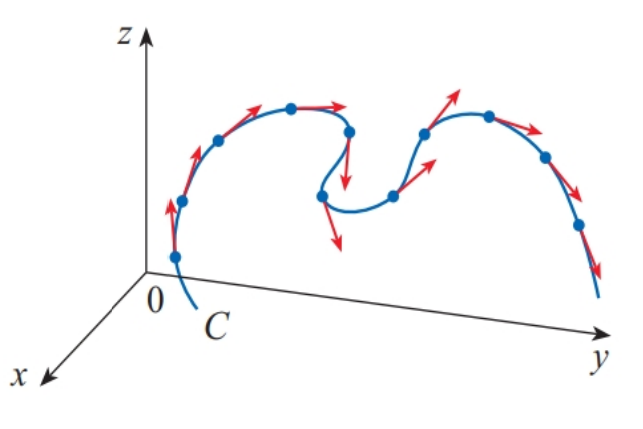
\includegraphics[scale=0.6]{figuras/vetor-tangente.png}
\end{center}
\newpage

A {\color{blue}curvatura} de $C$, em dado ponto, será definida de modo a medir

\begin{caixaazul}{}{}
{A taxa de variação da direção do vetor tangente unitário \textbf{\color{red}por unidade de comprimento}.}
\end{caixaazul}
Em outras palavras,
\begin{caixaazul}{}{}
{A medida de quão rapidamente a curva muda de direção no ponto}.
\end{caixaazul}

Por isso, definimos a curvatura como a norma  da taxa de variação do vetor tangente unitário com relação ao comprimento de arco, a saber,
\[
\kappa(s)=\left\|\frac{d\vec{T}(s)}{ds}\right\|,
\]
onde $\vec{T}$ é o vetor tangente unitário.

Entretanto, na maioria das vezes a curva não está parametrizada pelo comprimento de arco. Neste caso, podemos usar a Regra da Cadeia para obter uma fórmula em termos de um parâmetro qualquer. Se $s=s(t)$ é a função comprimento de arco, então:
\[\frac{d\vec{T}(s(t))}{dt}=\frac{d\vec{T}(s)}{ds}\frac{ds}{dt}=\frac{d\vec{T}}{ds}\|\vec{r}\,^\prime(t)\|.\]
Logo,
\[{\color{red} \kappa(t) =\frac{\|\vec{T}\,^\prime(t)\|}{\|\vec{r}\,^\prime(t)\|}.}\]

\begin{exeb}{}{}
Calcule a curvatura de um círculo de raio $\rho$.
\end{exeb}
\newpage

\marcador{subsection}{Vetores Normal principal e Binormal}


Como $\vec{T}$ é unitário, sabemos que $\vec{T}$ é ortogonal à  $\vec{T}\,^\prime$, portanto definimos o {\color{blue} vetor normal unitário principal} ou simplesmente  {\color{blue} vetor normal unitário} como
\[\color{red} \vec{N}(t)=\frac{\vec{T}\,^\prime(t)}{\|\vec{T}\,^\prime(t)\|}.\]
Veremos que este vetor indica a direção que na qual a curva está virando em cada ponto. A partir dele, definimos o {\color{blue} vetor binormal unitário}
\[\color{red} \vec{B}(t)=\vec{T}(t)\times \vec{N}(t).\]

\begin{center}
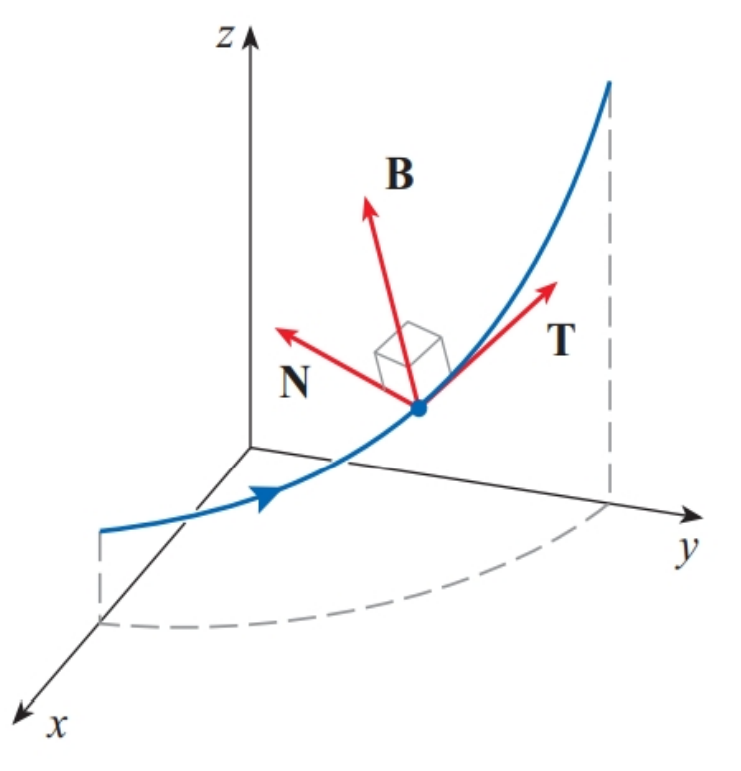
\includegraphics[scale=0.4]{figuras/normal-binormal.png}
\end{center}

Estes três vetores formam uma base ortonormal muito importante em geometria diferencial e no estudo de movimento de corpos, chamada de {\color{blue} Triedro de Frenet}.

\begin{exeb}{}{}
Determine os vetores normal e binormal da hélice circular $$\vec{r}(t)=(\cos(t),\sin(t),t).$$

\end{exeb}


